\documentclass[10pt, compress]{beamer}

\usetheme{metropolis}

\usepackage{booktabs}
\usepackage[scale=2]{ccicons}

%Icons
\usepackage{fontawesome}

%Syntax highlight
\usepackage{listings,xcolor}
\usepackage{inconsolata}

\definecolor{dkgreen}{rgb}{0,.6,0}
\definecolor{dkblue}{rgb}{0,0,.6}
\definecolor{dkyellow}{cmyk}{0,0,.8,.3}

% Language: PHP
\lstset{
  language        = php,
  basicstyle      = \small\ttfamily,
  keywordstyle    = \color{dkblue},
  stringstyle     = \color{red},
  identifierstyle = \color{dkgreen},
  commentstyle    = \color{gray},
  emph            =[1]{php},
  emphstyle       =[1]\color{black},
  emph            =[2]{if,and,or,else},
  emphstyle       =[2]\color{dkyellow}
}

%\usepgfplotslibrary{dateplot}


\title{Reverse engineering with determination}	
%\subtitle{}
\date{\today}
\author{Carl Svensson}
\institute{Securityfest 2017}

\begin{document}

\maketitle

\begin{frame}{About me}
  
	\begin{columns}
		\begin{column}{0.6\textwidth}  
  
  		\begin{itemize}
		  \item Carl Svensson, 26
		  \item MSc in Computer Science, KTH
		  \item Head of Security, Kry
		  \item CTF-player, HackingForSoju
		  \item \faEnvelope \hskip 2mm calle.svensson@zeta-two.com
		  \item \faTwitter \hskip 2mm  @zetatwo
		  \item \faGlobe \hskip 2mm https://zeta-two.com
		\end{itemize}
		
		\end{column}
		\begin{column}{0.4\textwidth} 
			\begin{center}
			
\includegraphics[width=0.4\textwidth]{images/kth.jpg}
			\end{center}
			\vspace{1cm}
			
\includegraphics[width=\textwidth]{images/kry_logo.png}
		\end{column}
	\end{columns}
  
\end{frame}

\begin{frame}{Reverse engineering in 30 seconds?}

 \begin{itemize}
  \item Take stuff, e.g. software, apart
  \item Understand how it works
  \item Many possible goals
    \begin{itemize}
  	\item Malware, what does it do?
  	\item Audit closed source components
    \end{itemize}  
  \item Static analysis
  \begin{itemize}
    \item + The whole picture
    \item - A lot to read, slow
  \end{itemize}  
  \item Dynamic analysis
  \begin{itemize}
    \item + See data flow
    \item - Not all paths taken
  \end{itemize}  
  \end{itemize}    

\end{frame}



\begin{frame}{Enter the M/o/Vfuscator}
  \begin{columns}
		\begin{column}{0.6\textwidth}
			\begin{itemize}
    \item x86 MOV is turing complete
    \item 1 instruction compiler
      \begin{itemize}
	  \item Chris Domas
	  \end{itemize}
    \item No branches
    \item Dummy data
  \end{itemize}
		\end{column}
		\begin{column}{0.4\textwidth}
			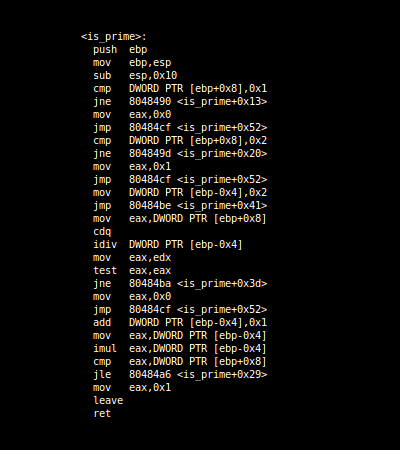
\includegraphics[width=0.9\textwidth]{images/gcc_asm.png}
			\linebreak
			\linebreak
			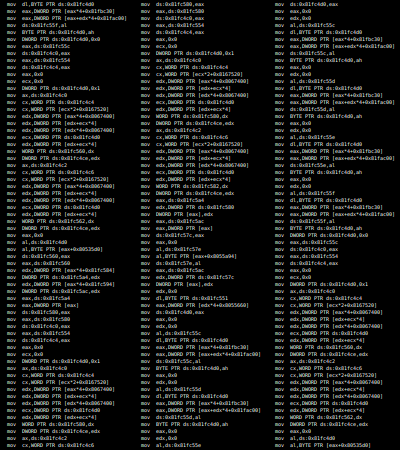
\includegraphics[width=0.9\textwidth]{images/mov_asm.png}
		\end{column}
	\end{columns}

  
\end{frame}

\begin{frame}{Crack Me \#1}
  \begin{itemize}
    \item Find the password
    \item Dead ends
    \begin{itemize}
      \item Name functions
      \item Study branches
      \item Trace execution
      \item Count instructions
    \end{itemize}
  \end{itemize}
\end{frame}

\begin{frame}{Intermission: What is a program?}
  \begin{itemize}
    \item Takes input
    \item Perform calculations
    \item Affects the world   
    \begin{itemize}
      \item Output
      \item Affect memory
      \item OS API calls
    \end{itemize}
  \end{itemize}
\end{frame}

\begin{frame}{Crack Me \#1, take 2}
	\begin{itemize}
    \item Memory trace
    \item Diff
    \item Scripting glue
    \item Victory!
    \end{itemize}
\end{frame}

\begin{frame}{Electronics 101}
\begin{columns}
		\begin{column}{0.6\textwidth}
	\begin{itemize}
	\item Boolean circuits
	\item Gates
	\begin{itemize}
	  \item AND, OR, NOT, NAND, XOR
	  \item D-latch, Flip-Flip
	\end{itemize}
	\item Functional completeness
	\end{itemize}
	\end{column}
		\begin{column}{0.4\textwidth}
			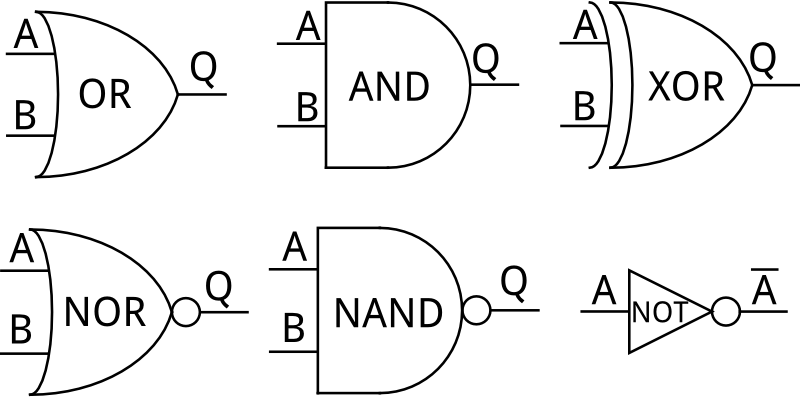
\includegraphics[width=1\textwidth]{images/gates.png}
			\linebreak
			\linebreak
			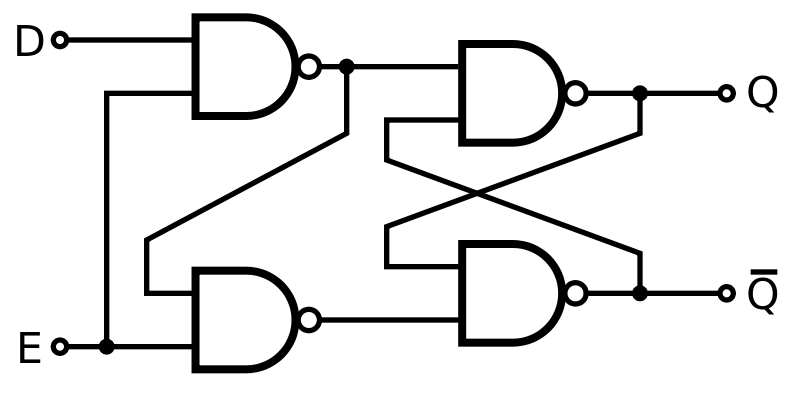
\includegraphics[width=1\textwidth]{images/d-latch.png}
		\end{column}
	\end{columns}

\end{frame}

\begin{frame}{Crack Me \#2}
\begin{columns}
		\begin{column}{0.5\textwidth}
	\begin{itemize}
	\item Keypad, IC \& lock
	\item Single "instruction"
	\item Easy way: dynamic
	\item My way: static
		\begin{itemize}
		\item Find subgraph
		\item Replace, abstract, iterate
		\item Naming
		\end{itemize}
	\end{itemize}
	\end{column}
		\begin{column}{0.5\textwidth}
			\includegraphics[width=1\textwidth]{images/schematic.png}
		\end{column}
	\end{columns}
\end{frame}


\begin{frame}[standout]
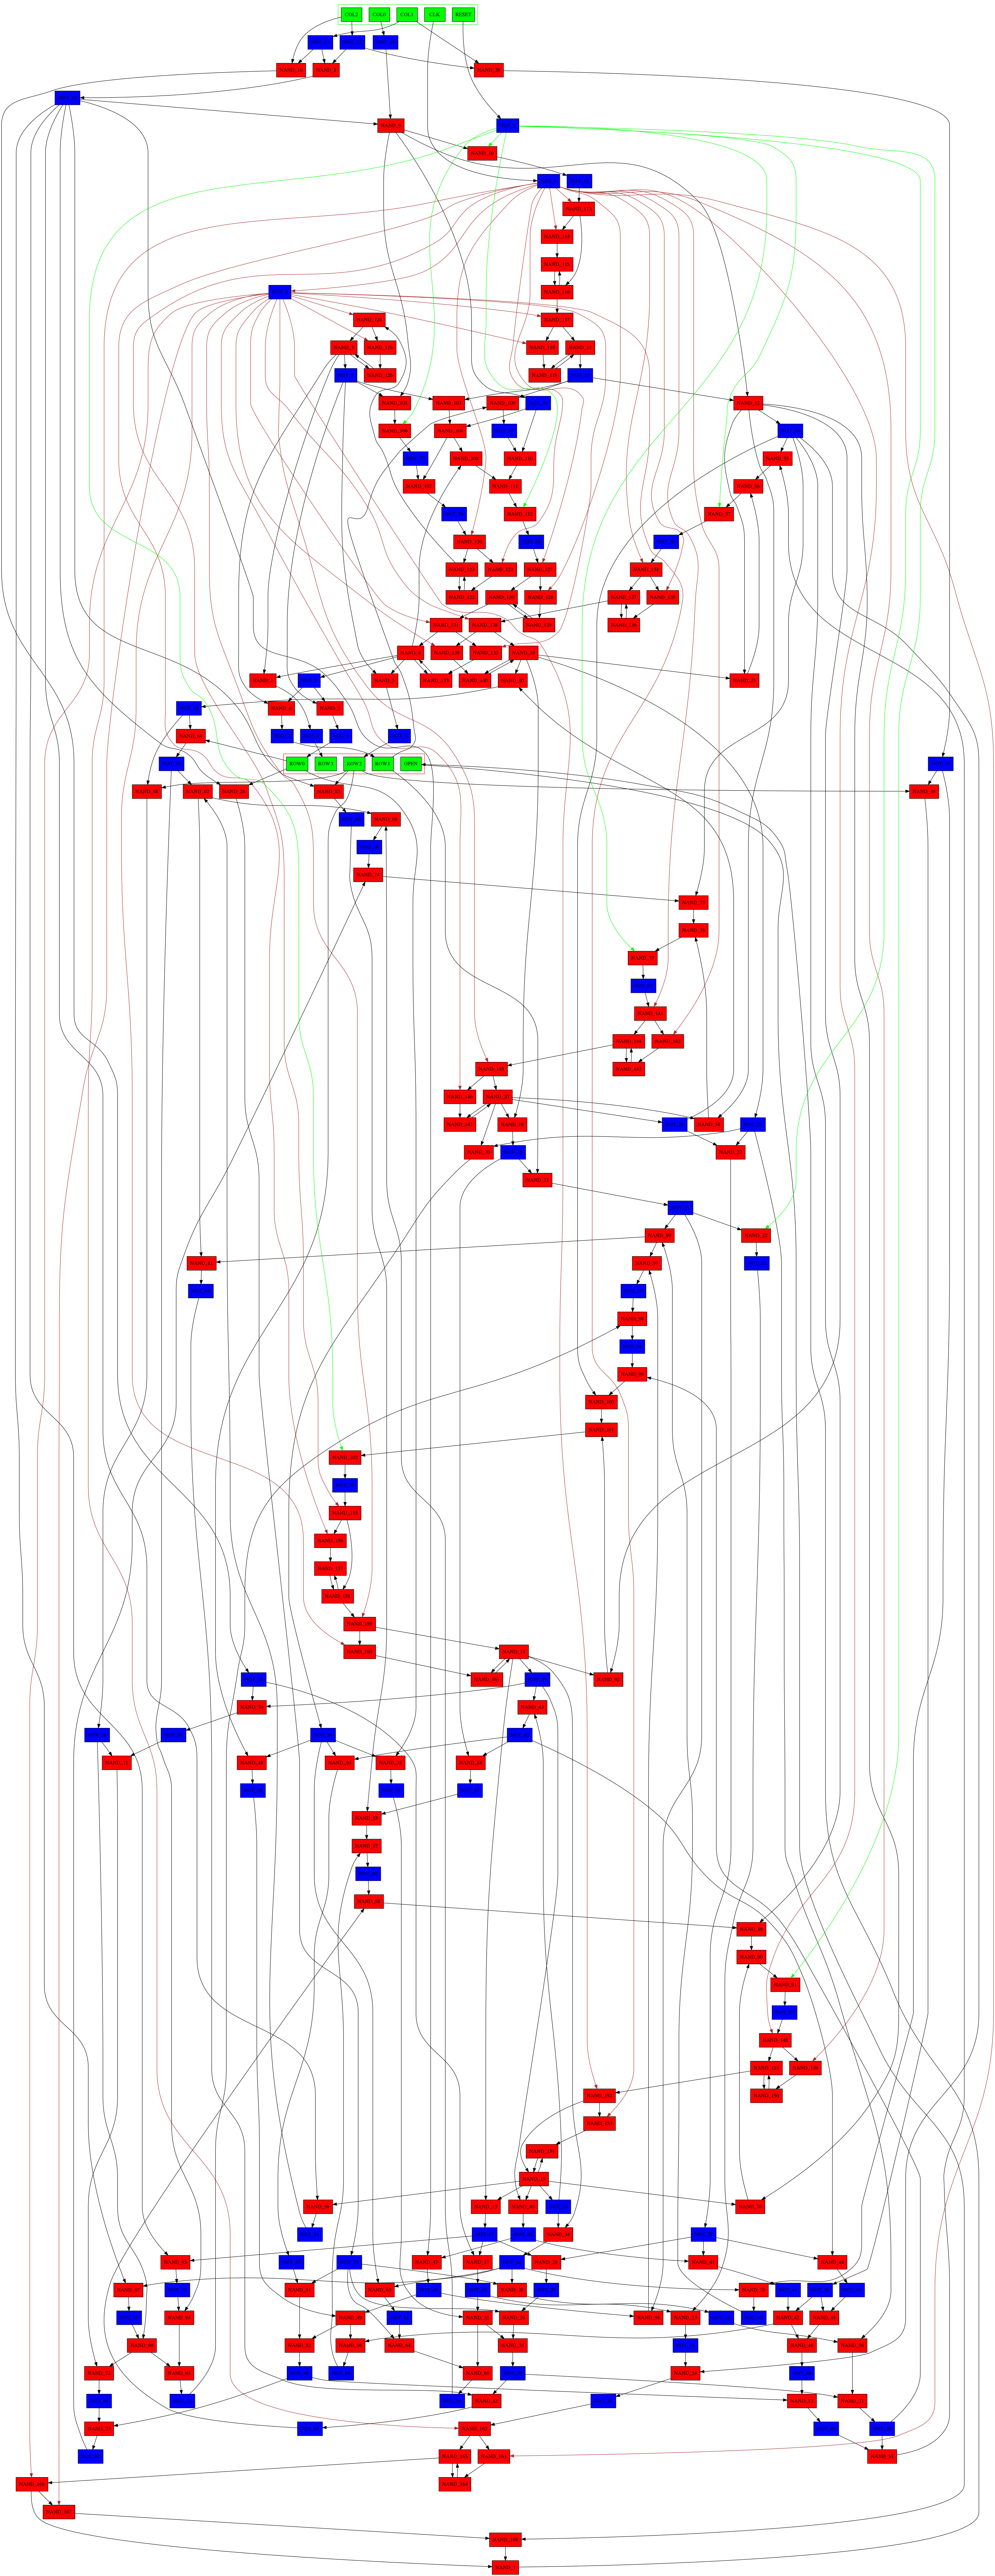
\includegraphics[width=1\textwidth]{images/netlist1_full.png}
\end{frame}


\begin{frame}[standout]
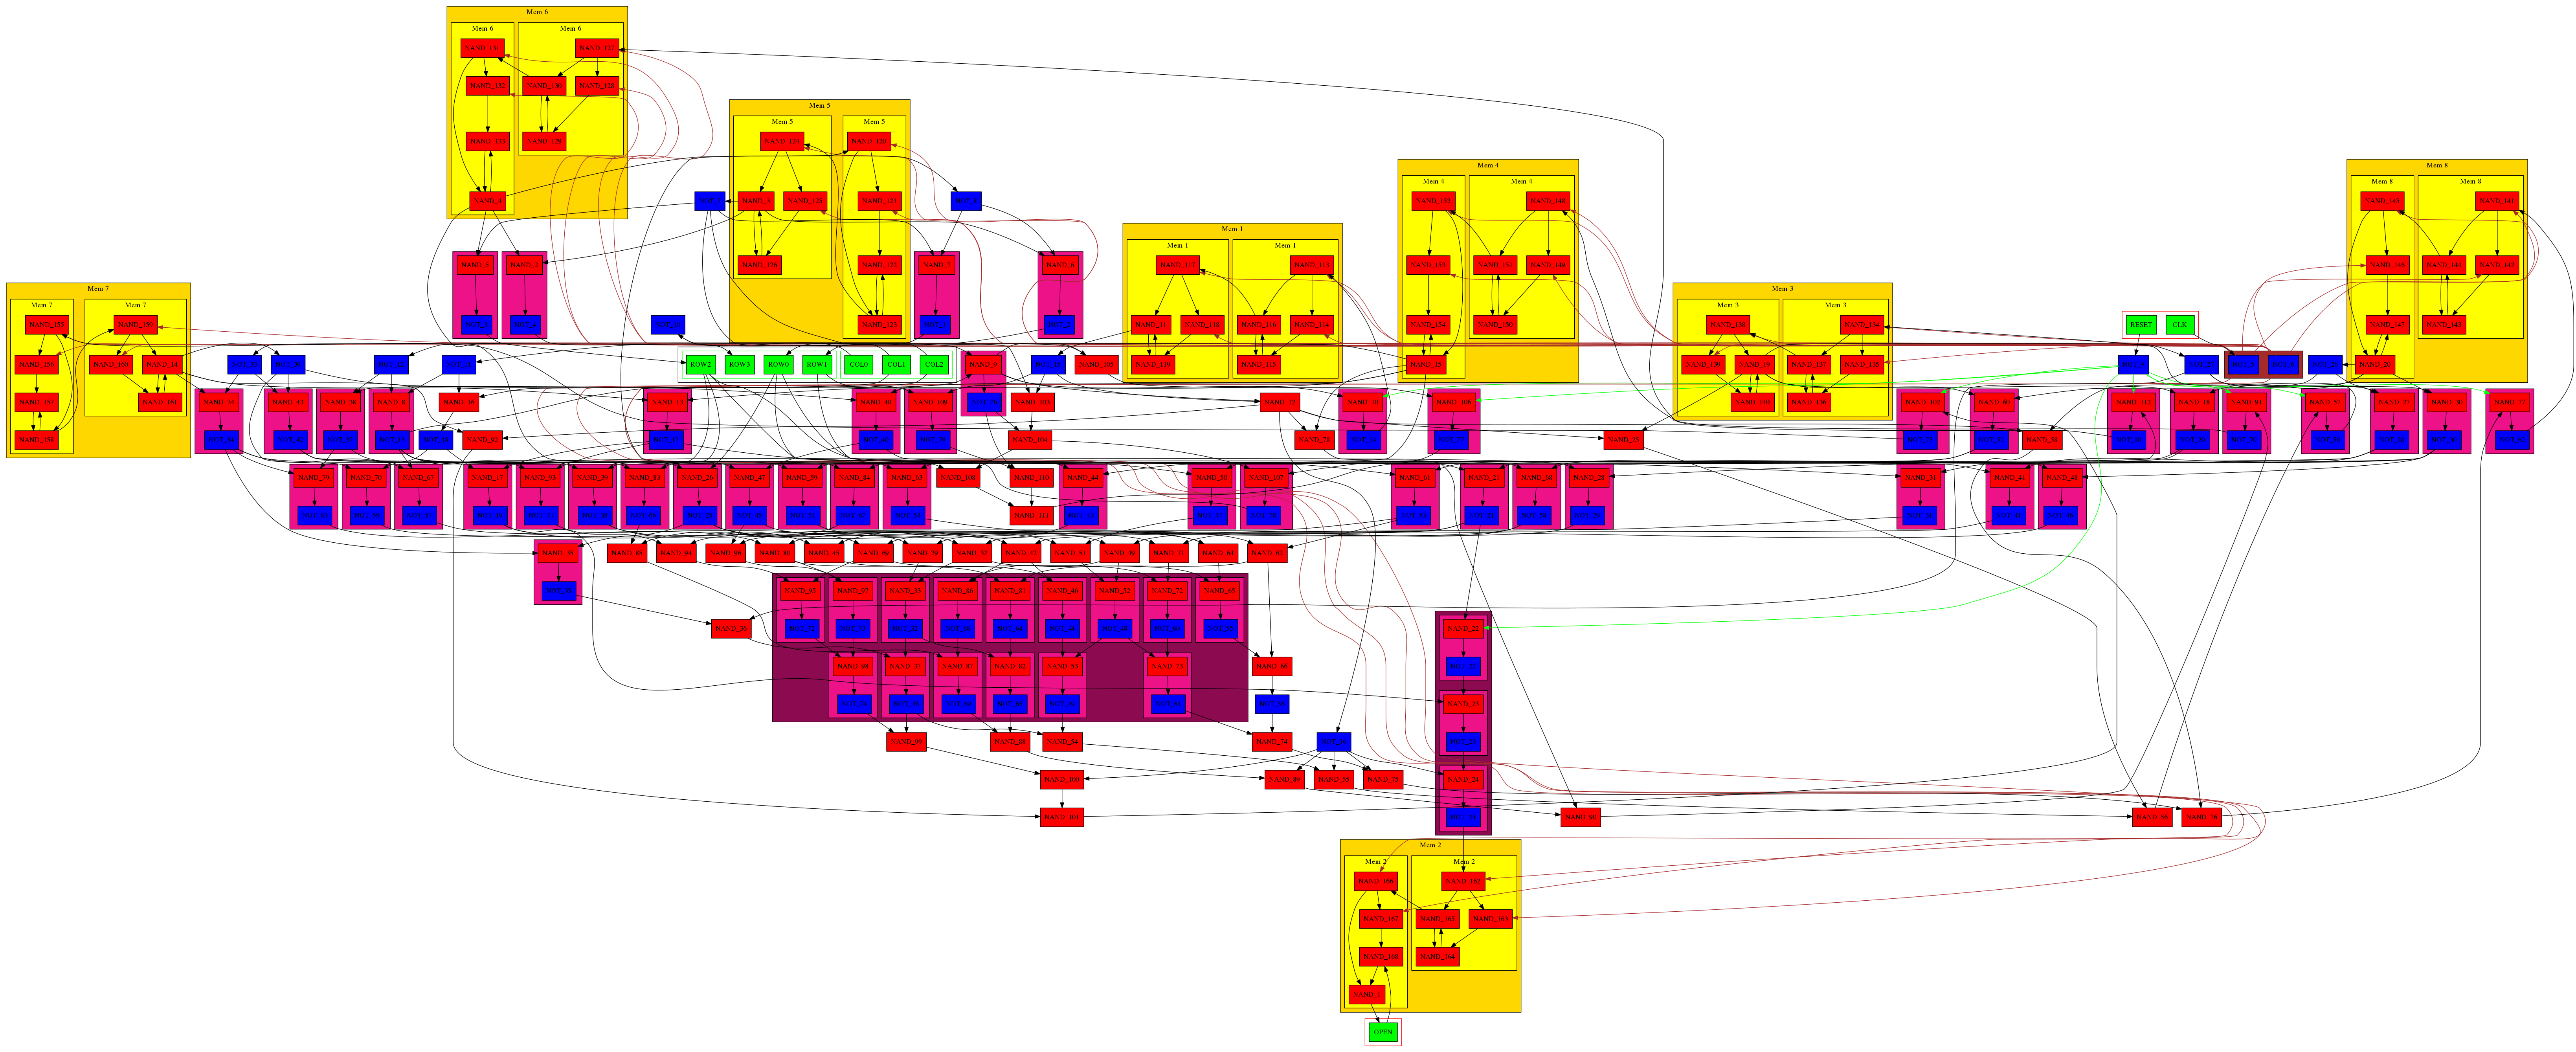
\includegraphics[width=1\textwidth]{images/netlist2_grouped.png}
\end{frame}

\begin{frame}[standout]
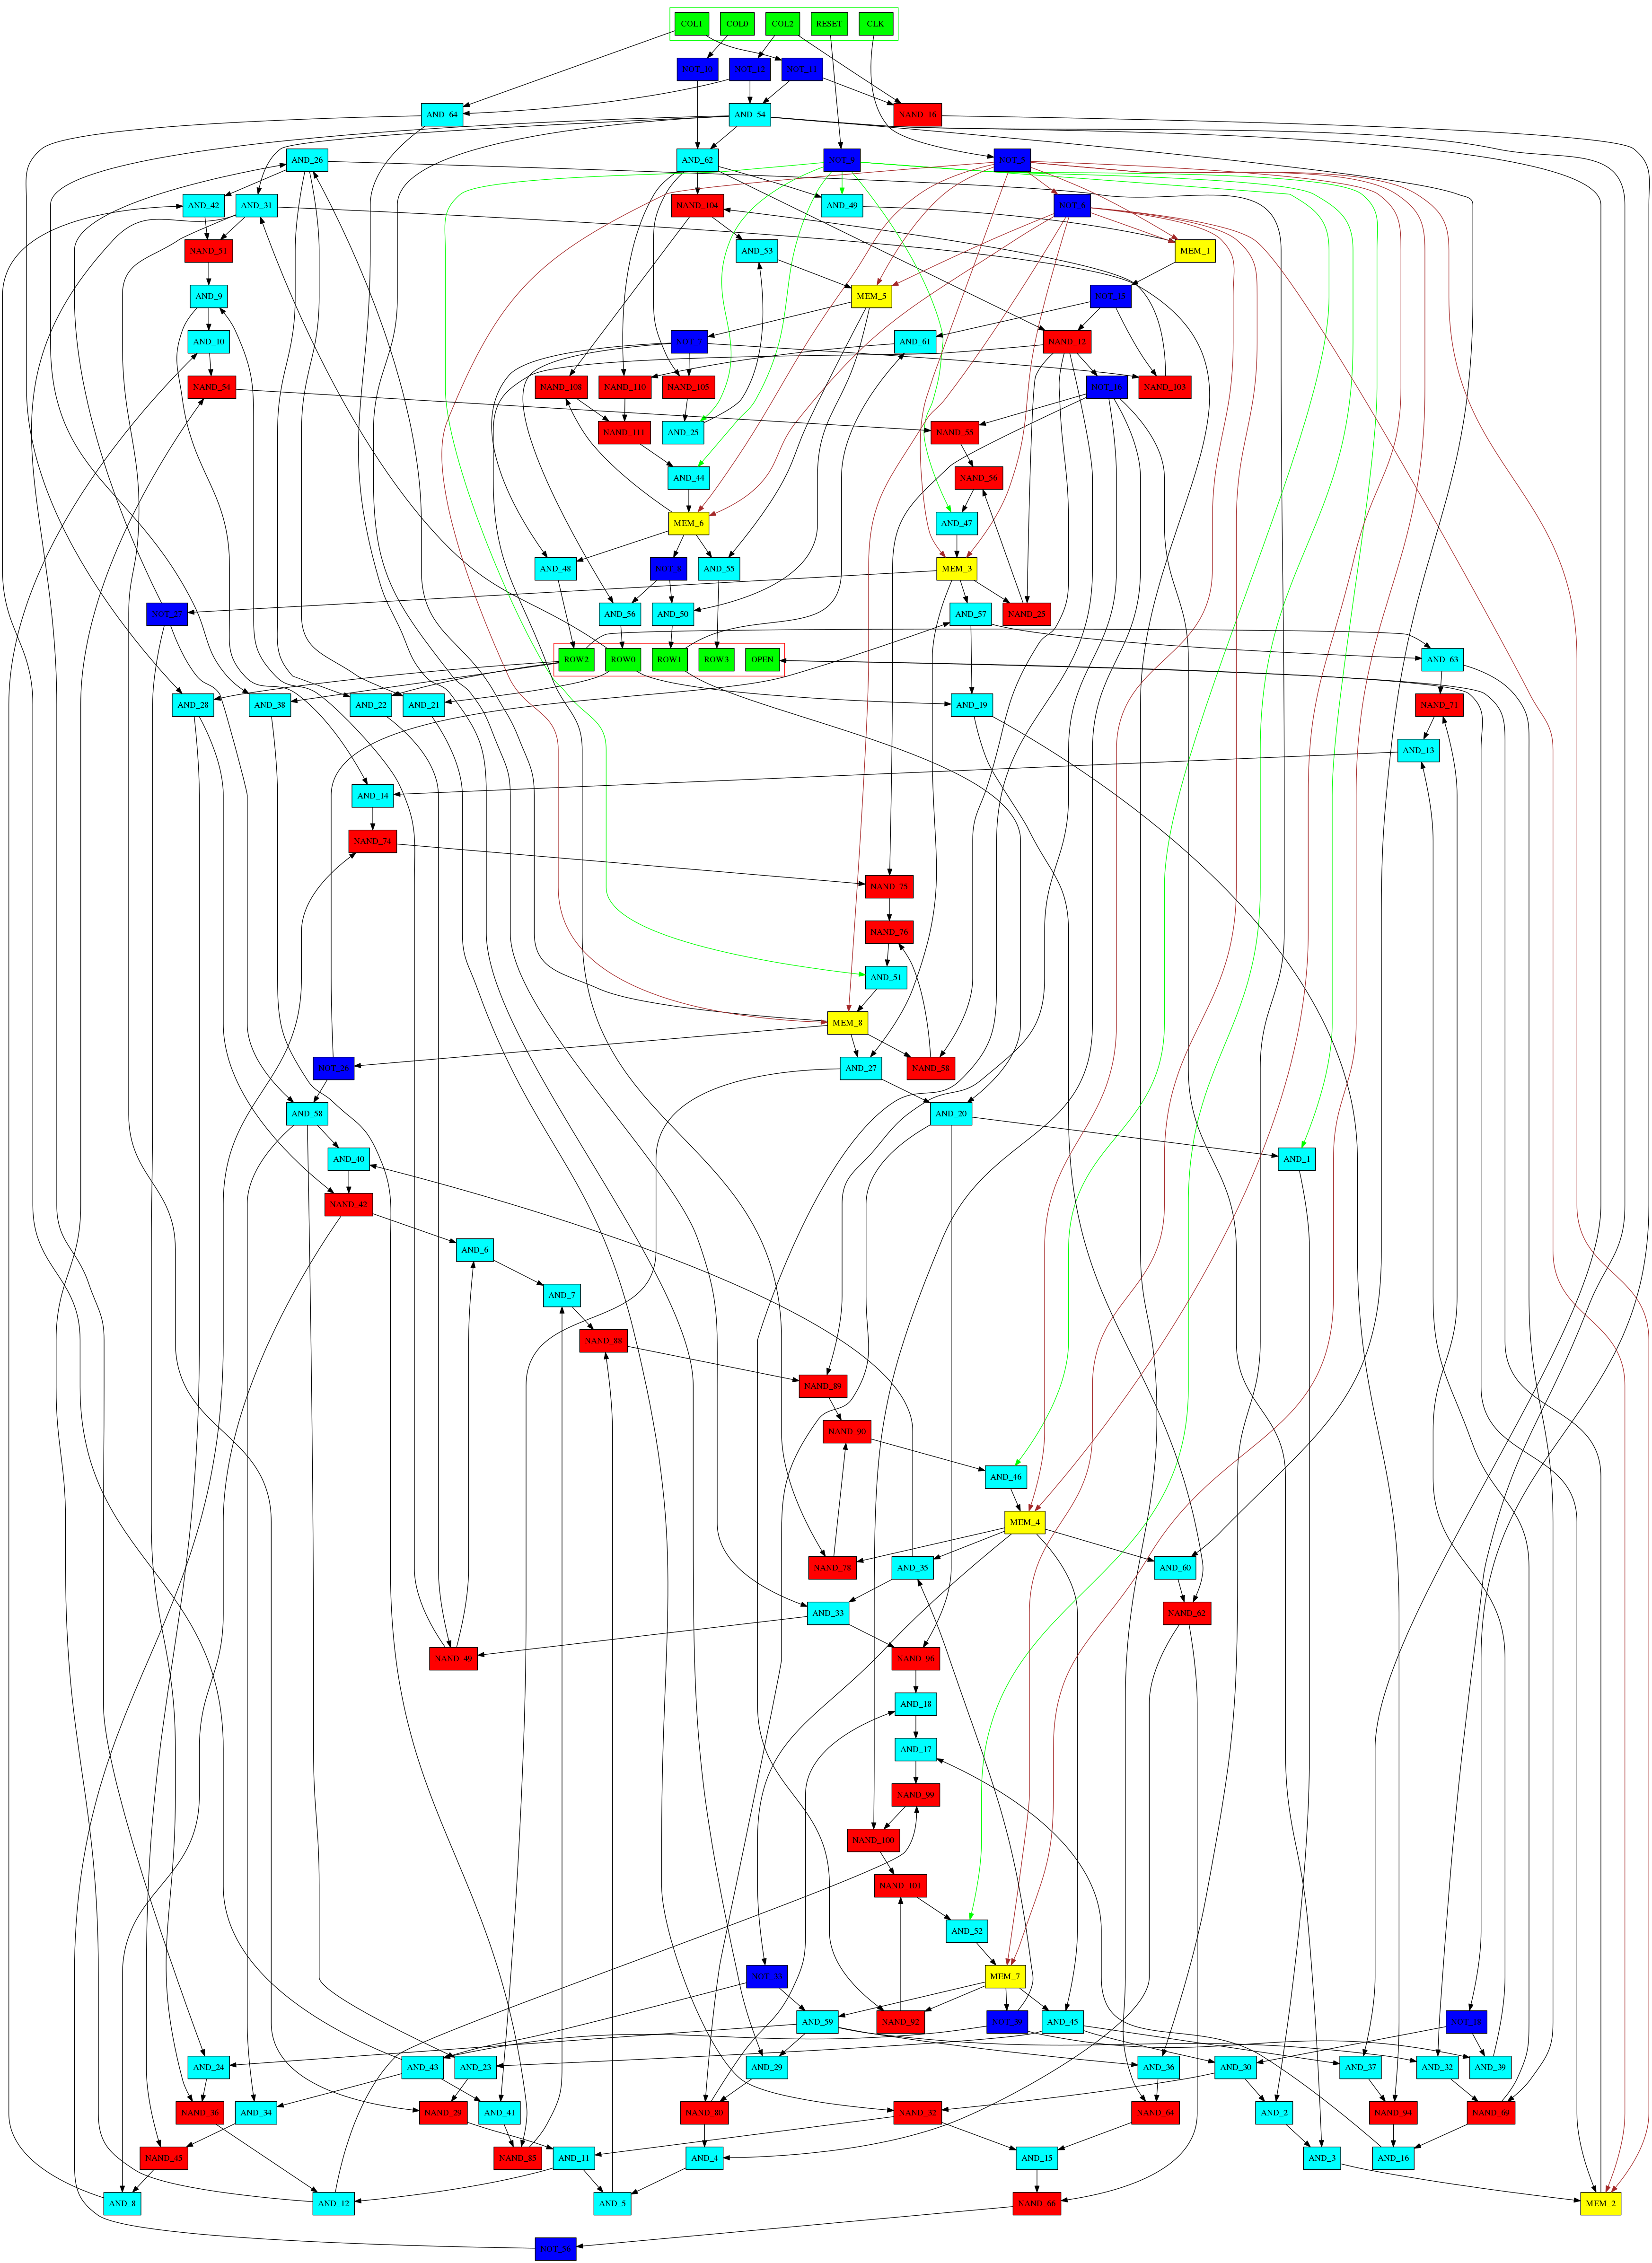
\includegraphics[width=1\textwidth]{images/netlist3_replaced.png}
\end{frame}

\begin{frame}[standout]
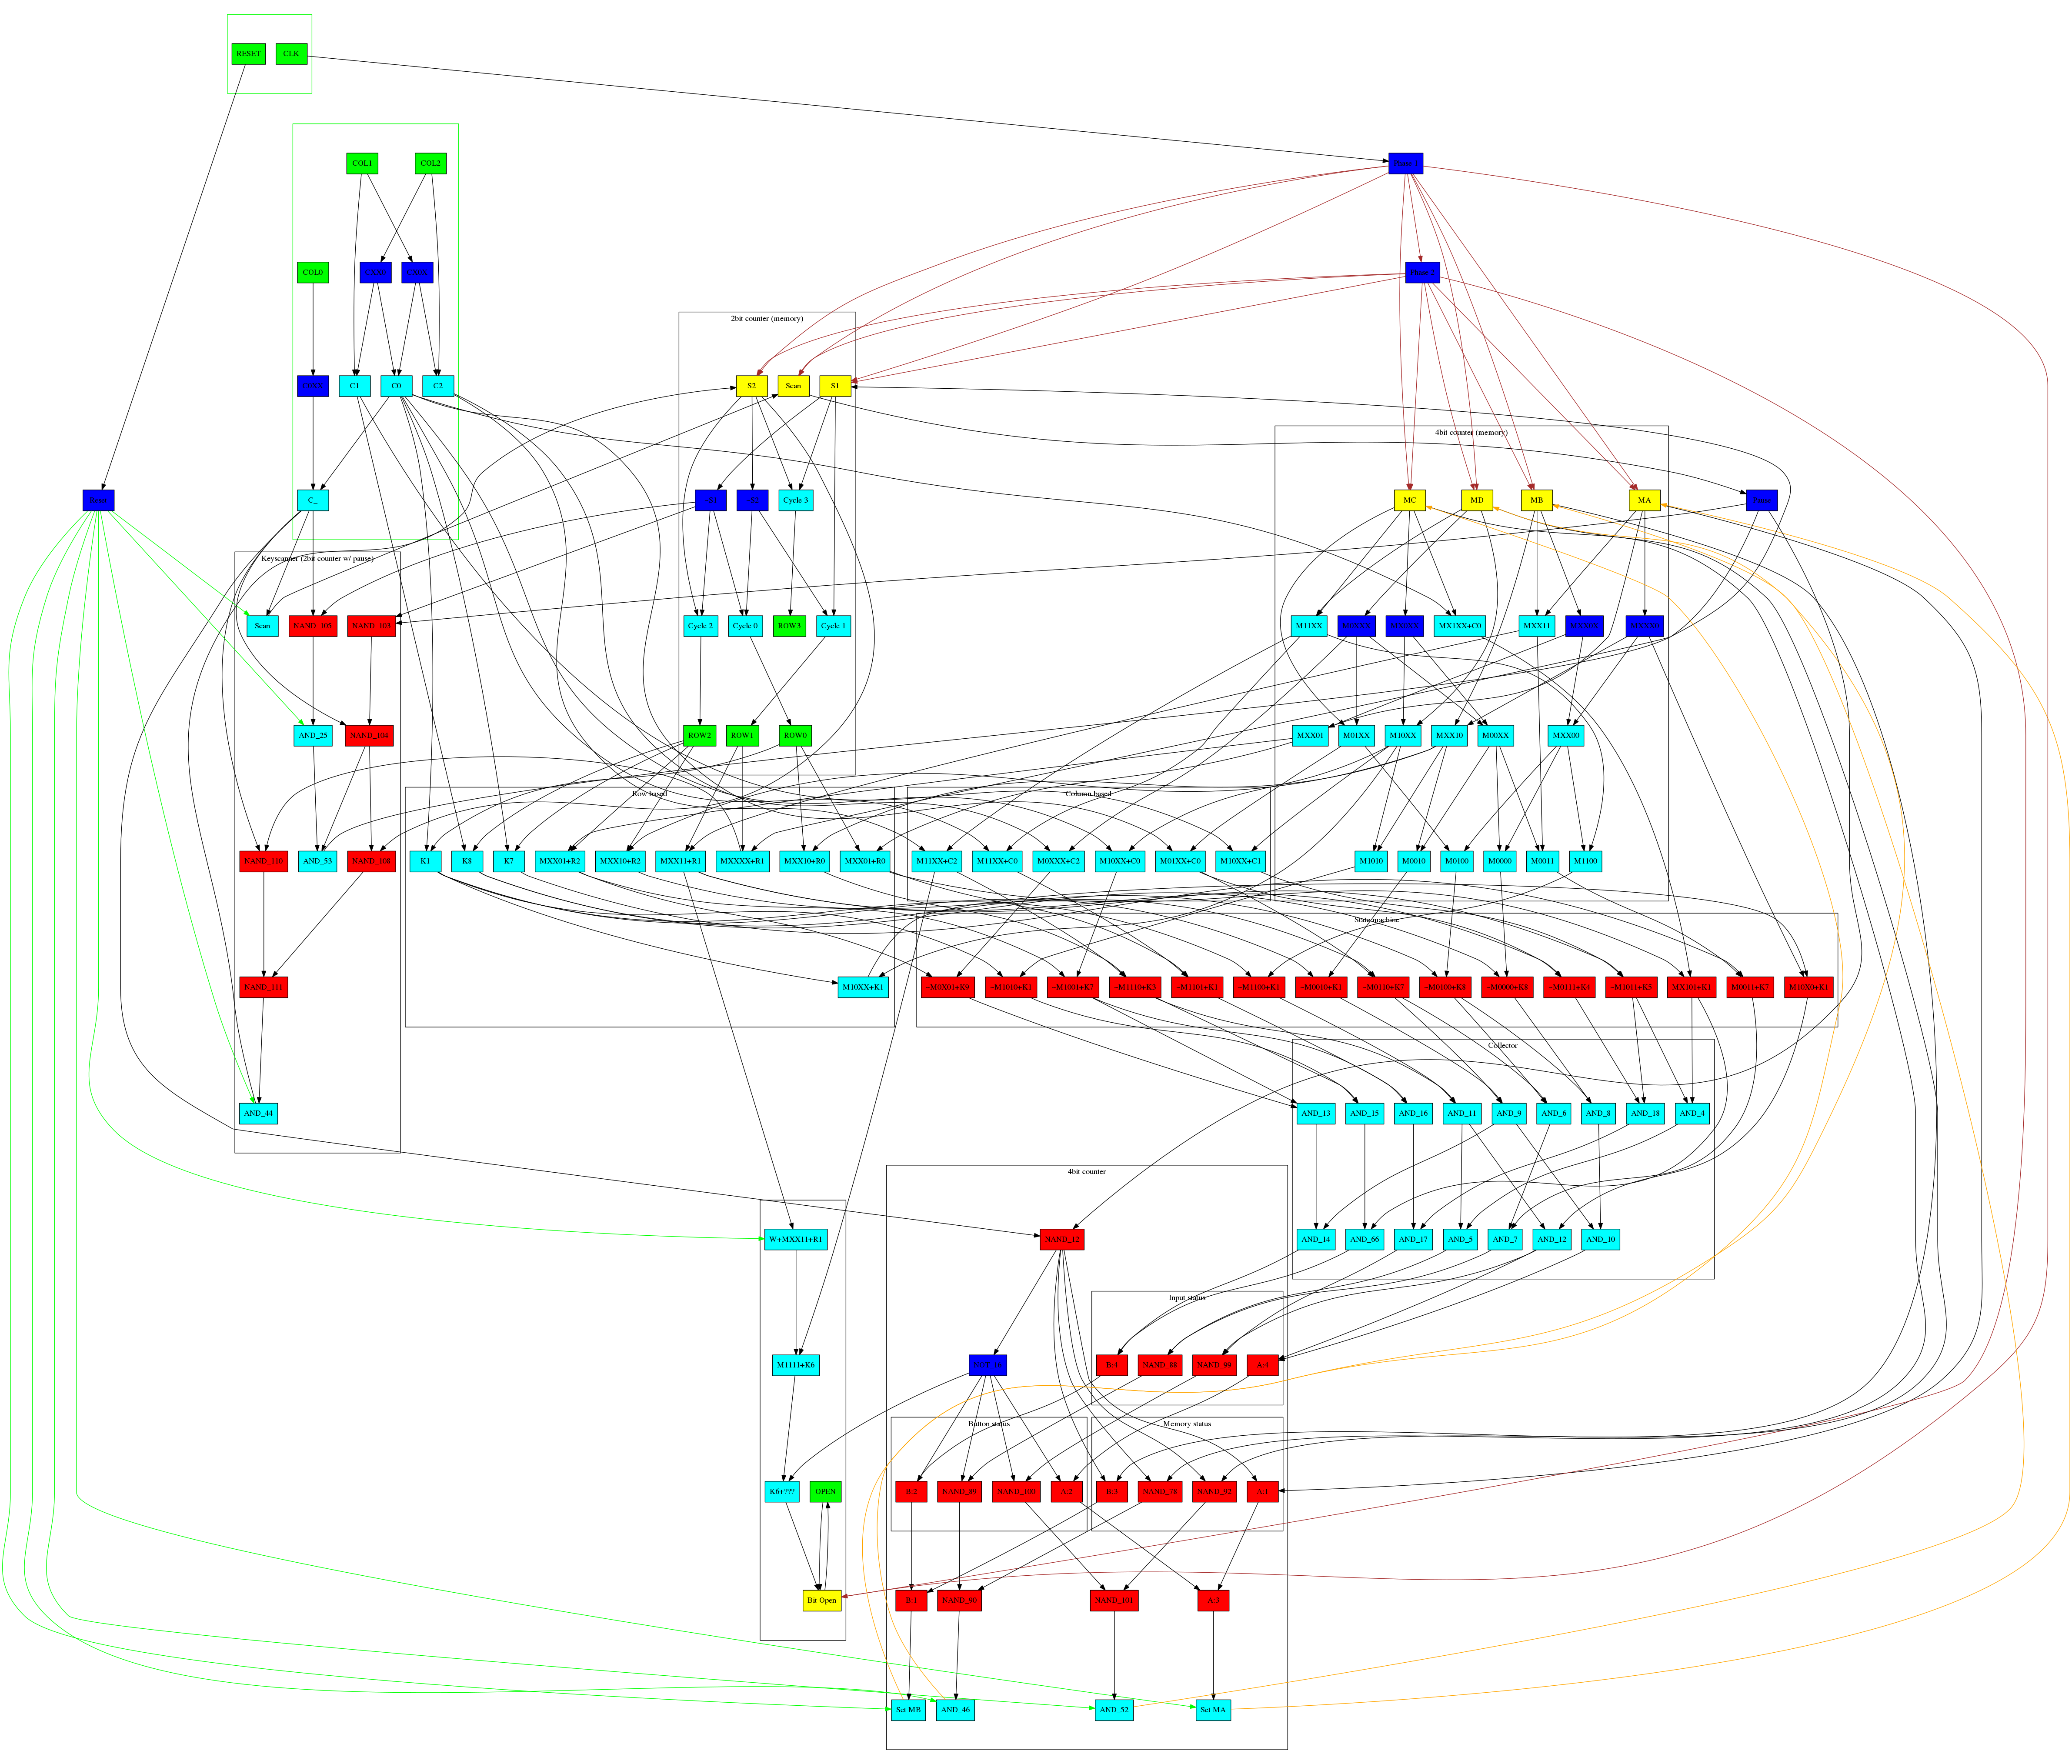
\includegraphics[width=1\textwidth]{images/netlist4_abstract.png}
\end{frame}


\begin{frame}{Keep practicing, stay sharp}
	\begin{itemize}
		\item Like going to the gym
		\item Push your limits
		\item Have fun!
		\item LabyREnth, http://labyrenth.com/ 10/6-23/7
			\begin{itemize}
			\item \$23,000 USD total prizes
			\end{itemize}
	\end{itemize}
\end{frame}

\begin{frame}[standout]
Thanks for listening!
\end{frame}



\end{document}
